In the 19\textsuperscript{th} and early 20\textsuperscript{th} century, birds of prey became victims of human attempts to control nature, being perceived as a danger and competition. They were severely threatened by pesticides, systematically persecuted, poisoned and their nests were looted \parencite{aebischer2021rotmilan, collar1988birds, ntampakis2005red}. The ecological problems posed by this targeted persecution were recognised in the second half of the 20\textsuperscript{th} century and the importance of functioning conservation was understood, which is fundamental for population recovery \parencite{aebischer2021rotmilan, seoane2003effects}. The red kite (\textit{Milvus milvus}), as a European bird of prey, has also undergone this development and was considered almost extinct towards the end of the 19\textsuperscript{th} century, before gradually recovering in recent decades and now being classified as "Least Concern" in the European Red List of Birds \parencite{birdlife2021redlist}. The current population of red kites is estimated at about 60'000 to 70'000 individuals with around 35'000 breeding pairs, the majority of which are found in Germany (14'000-16'000 pairs), U.K (4'388 pairs), Sweden (3'100-4'100 pairs), France (3'000-3'900 pairs), Switzerland (2'800-3'400 pairs) and Spain (2'312-2'440 pairs), meaning that these six countries account for over 90\% of the world population \parencite{birdlifefactsheet}. Due to this remarkable development, there are numerous studies devoted to the red kite. In the following sections, the ecology of the red kite is examined in more detail, and finally the history and various aspects of the research field of movement ecology are discussed.

\subsection{Red Kite Ecology}
\subsubsection{Appearance}
The red kite is a bird of prey native to Europe \parencite{garcia2022seasonal, literak2022disperal, panter2022age}. Despite its impressive wingspan of over 1.5 meters, it weighs only about 1 kg \parencite{aebischer2021rotmilan, ortlieb1989rotmilan}. Its appearance is unmistakable with its long wings, forked tail and distinctive rusty brown ground colouring. The head and parts of the underside of the flying bird stand out from the ground colouring in a whitish grey tone. Red kites show a weak sexual dimorphism, which is why sex is often determined genetically. \parencite{aebischer2021rotmilan}. Two examples of a flying red kite are shown in Figure~\ref{figure:red_kites}, once from the underside and once from the top.

\vspace{1\baselineskip}

\begin{figure}[H]
\centering
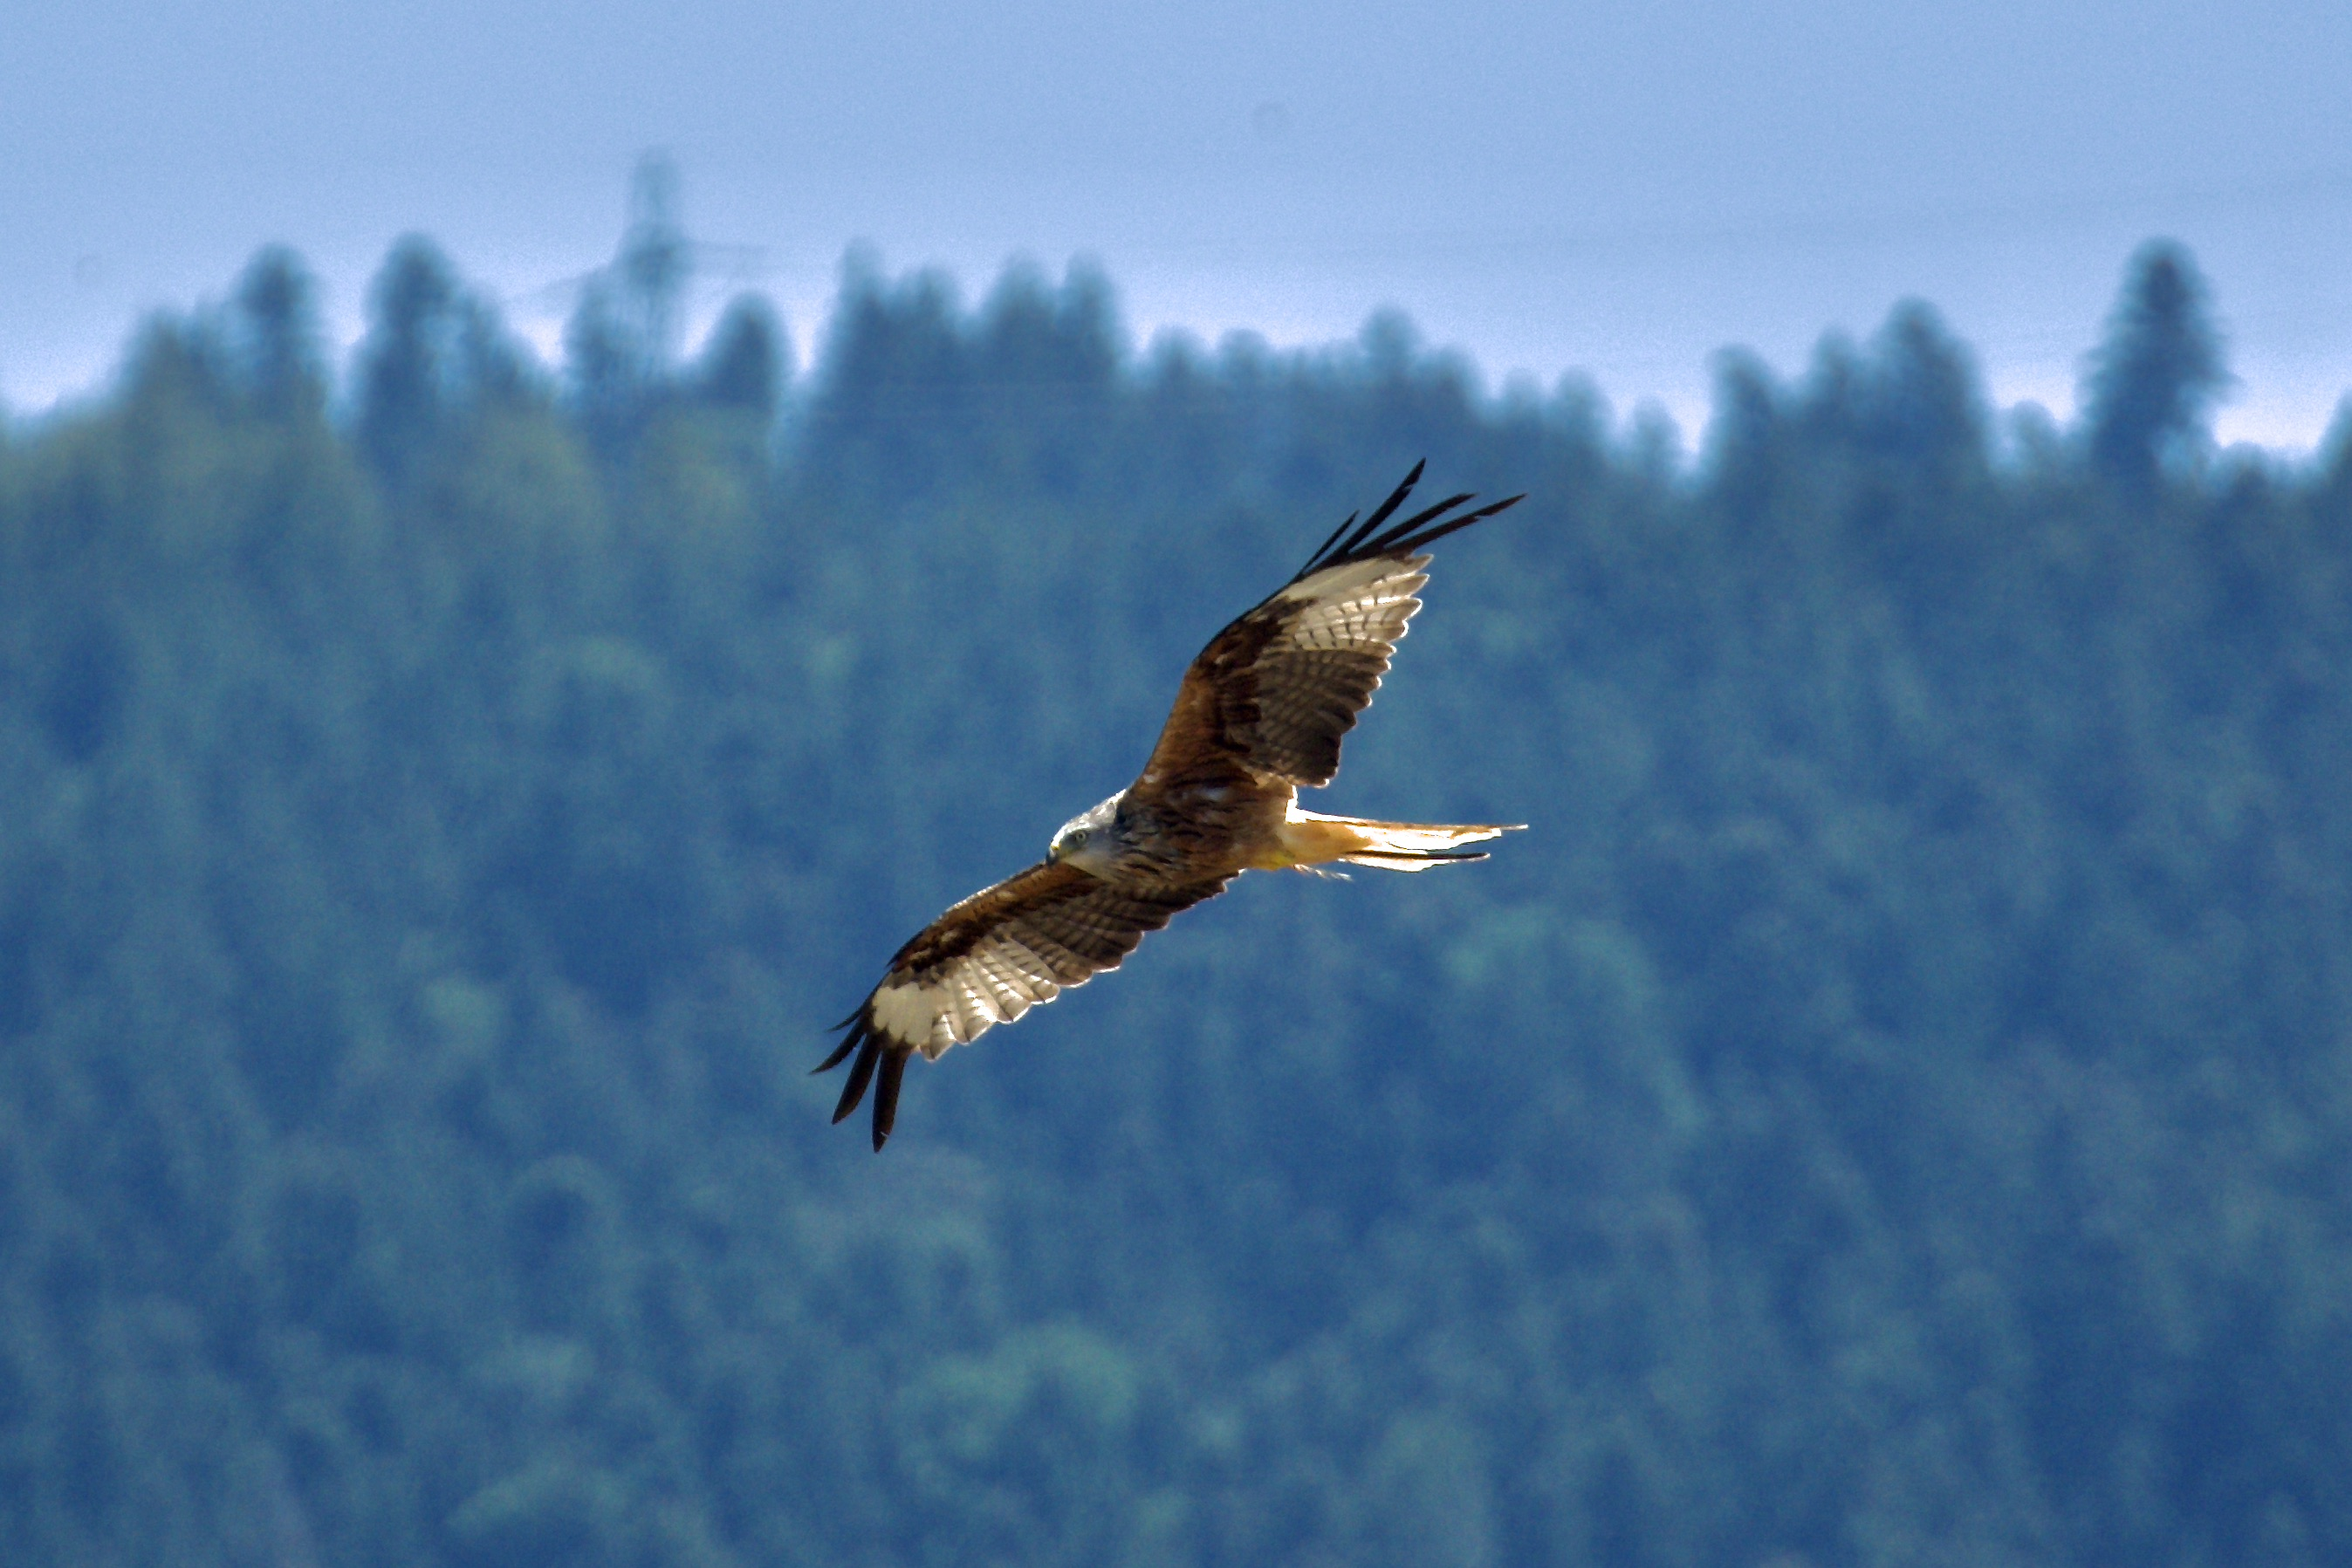
\includegraphics[width=0.495\textwidth]{figures/background/Red_kite_bottom.jpeg}
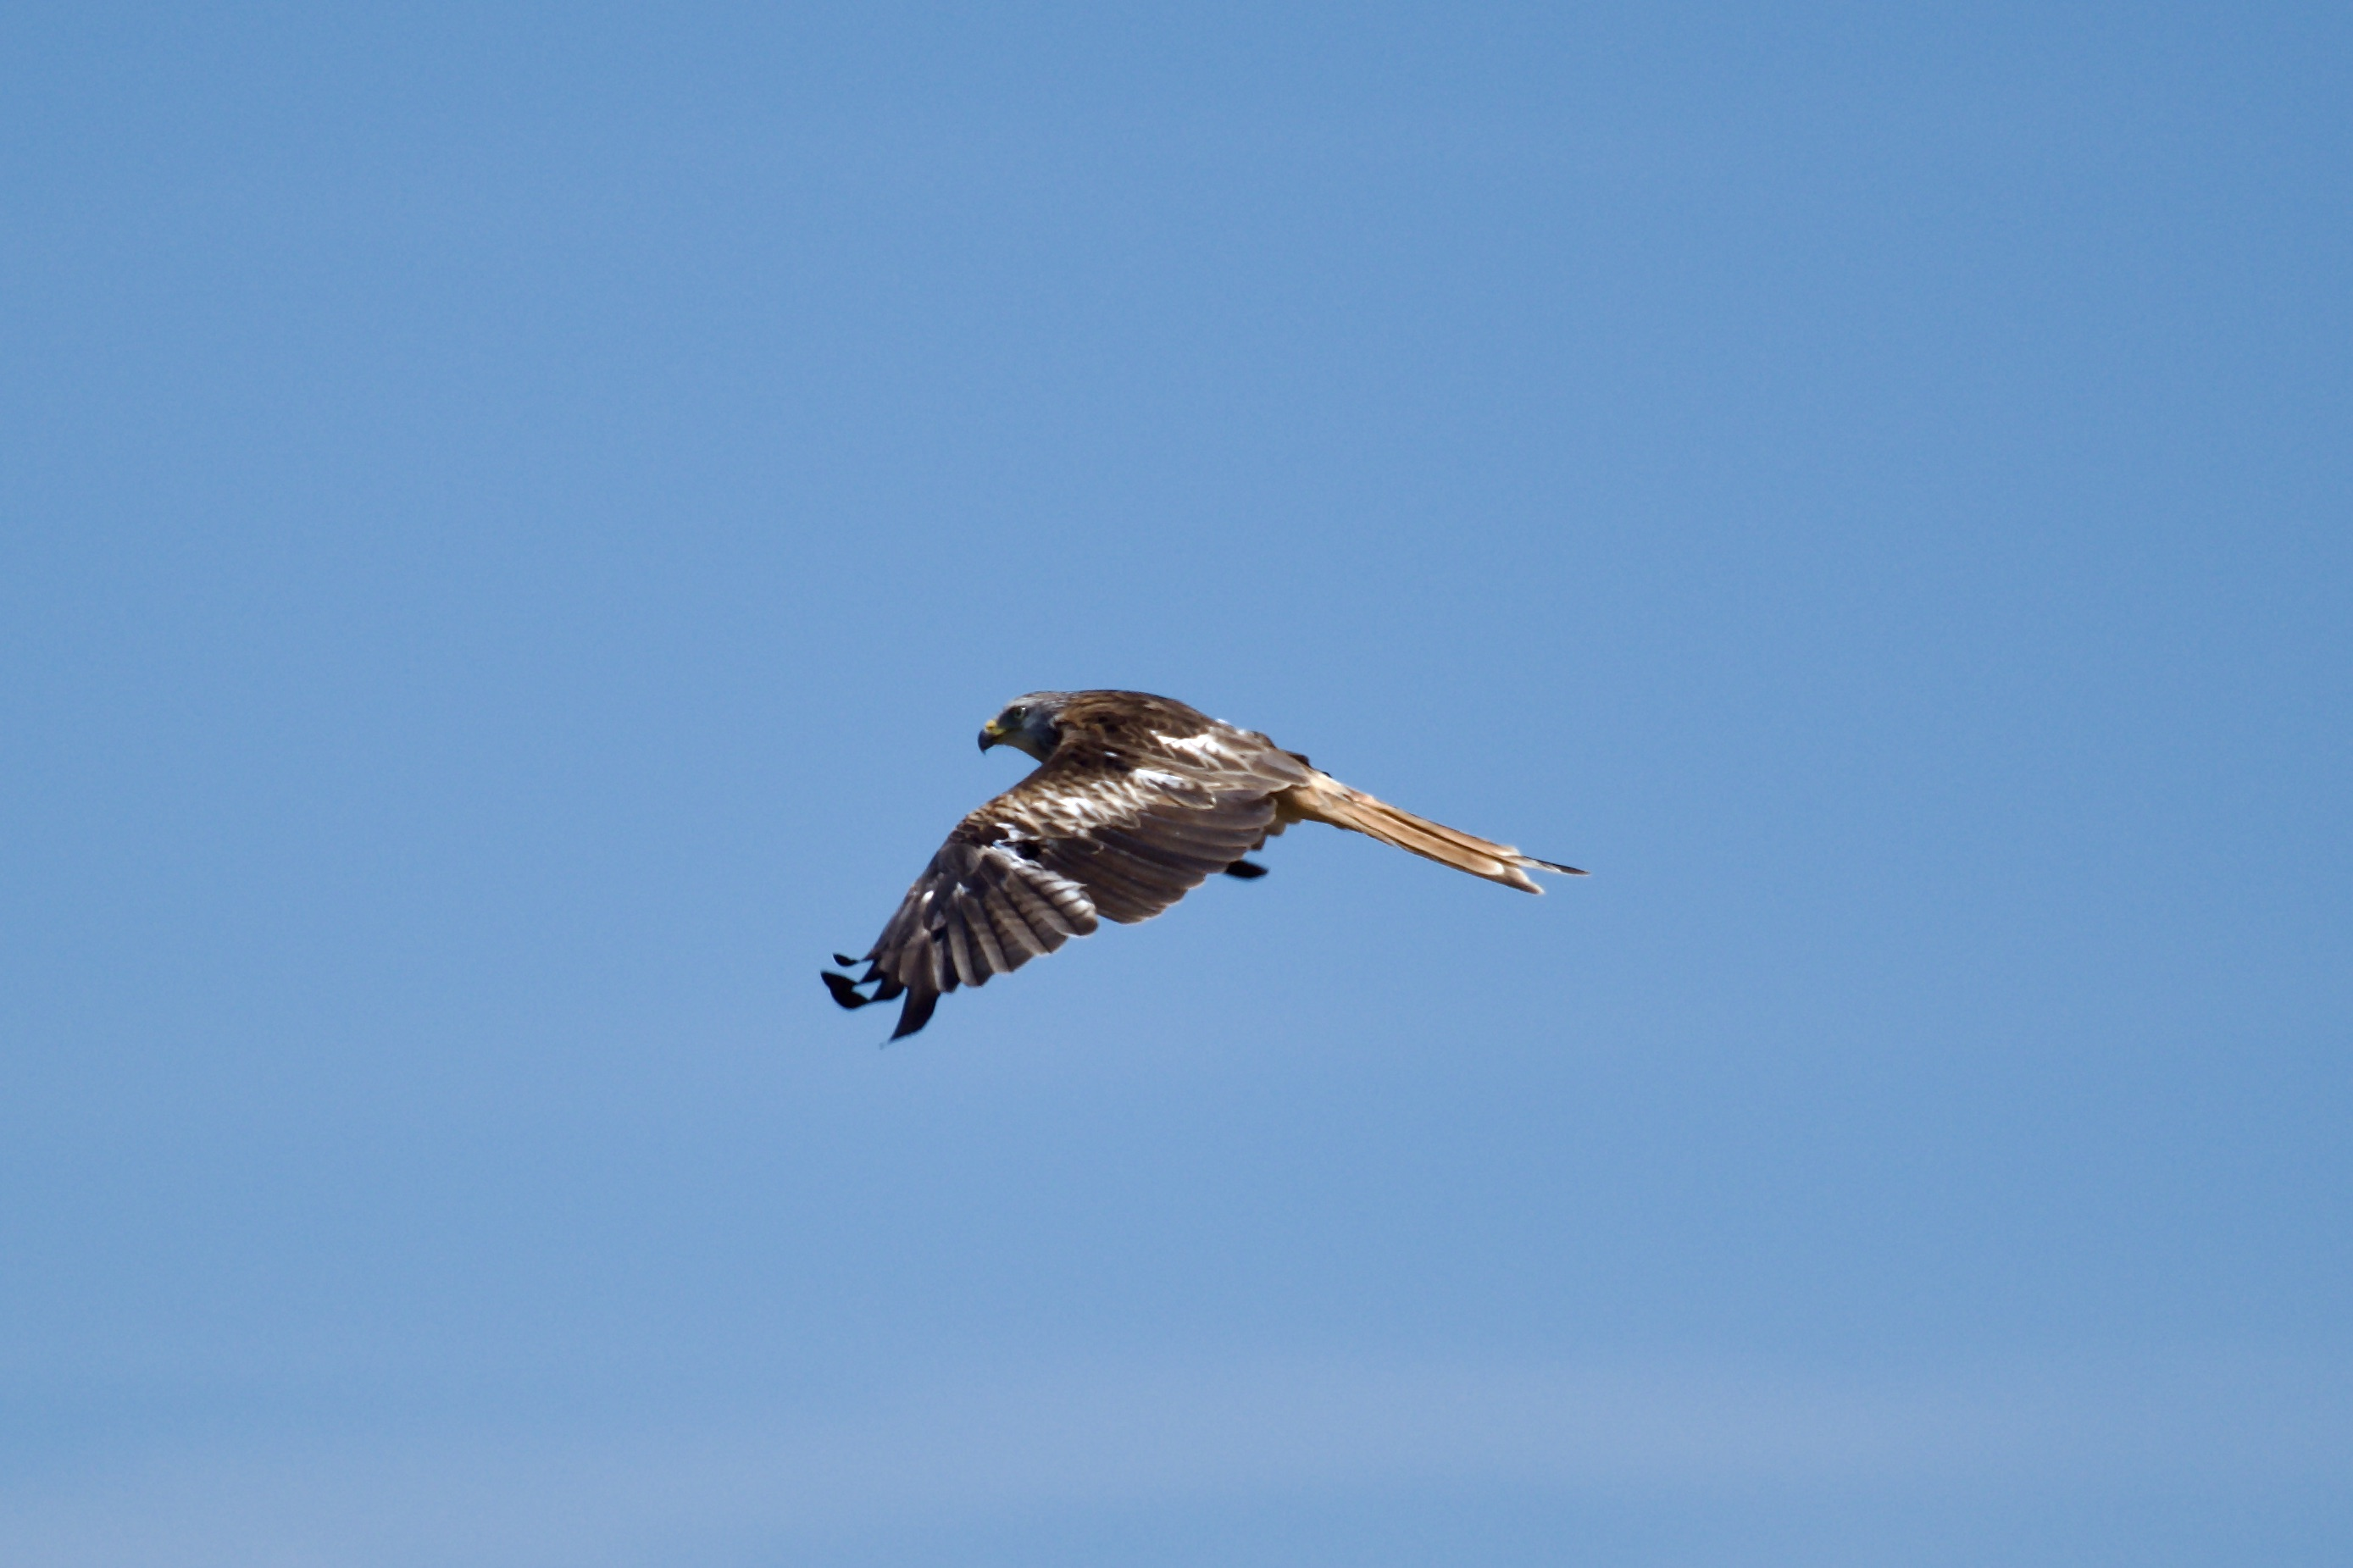
\includegraphics[width=0.495\textwidth]{figures/background/Red_kite_top.jpeg}
\caption[Red kites in flight]{Red kites in flight. Image credit: U. Beeli.}
\label{figure:red_kites}
\end{figure}

\subsubsection{Habitat}
Red kites hunt in open areas and nest in tall trees, which is why they prefer diversely structured cultural landscapes with fields and fragmented forest \parencite{mougeot2011breeding}. Red kites mainly prey on small mammals and are opportunistic scavengers, feeding on a wide range of prey, also including worms, insects, fish, birds, reptiles, amphibians, and anthropogenic food \parencite{aebischer2021rotmilan, cereghetti2019quantification, orros2015widespread, welti2019carcass}. Due to the wide prey spectrum, it is likely that red kites may be less susceptible to natural fluctuations in certain food sources \parencite{aebischer2021rotmilan, mougeot2011breeding}.

\subsubsection{Life History}
Red kites show a high variability between individuals in migration behaviour, with some individuals migrating while others remain stationary, known as partial migration \parencite{garcia2022seasonal, jaffre2013long}. Migrating birds begin the autumn migration to their wintering areas from August to November \parencite{aebischer2021rotmilan, garcia2022seasonal, pfeiffer2009satelliten}. Birds breeding in northern Europe tend to show a migratory behaviour and spend the winter months in southern Europe, mainly in southern France, on the Iberian Peninsula, in Italy and in Balkan regions as far as Greece \parencite{ferreira2015wintering, garcia2022seasonal, maciorowski2019autumn, mougeot2011breeding, panter2022age}. Birds breeding in southern Europe mostly remain in the Mediterranean region throughout the year \parencite{crespo2020analysis}, which is mainly due to the milder climate and the sufficient resource availability, making overwintering possible \parencite{garcia1998geographic}. Also in Central Europe there is an increasing number of individuals that overwinter locally and no longer migrate to southern areas \parencite{aebischer2021rotmilan}. After wintering, migrating birds begin the spring migration to their breeding areas from February to April \parencite{aebischer2021rotmilan, garcia2022seasonal, pfeiffer2009satelliten}. Red kites usually breed for the first time at the age of three to four years, but there are exceptions that start at the age of one or two years, as well as those that start later \parencite{mougeot2011breeding}. Once a breeding pair has found a home range, it is faithful to both the pair-member and the home range \parencite{aebischer2021rotmilan, mougeot2011breeding, scherler2023brutbiologie}.

\subsubsection{Reproduction} \label{reproduction}
Red kites begin to occupy their home ranges as early as February, but often not before March \parencite{aebischer2021rotmilan}. The area over which red kites forage for nesting material and food is highly dependent on habitat quality, sex and season, and can therefore vary greatly from one area to another \parencite{spatz2022sex}. Red kites do not claim a large territory exclusively, but they defend their nest fiercely against intruders from about 50-100m \parencite{aebischer2021rotmilan}. For this reason, it will be referred to a bird's activity range as its home range in this work. It is not trivial to determine the typical home range size of red kites, as there is great variability between individuals and regions. Home range sizes of 8.7--38.4 km$^2$ for males and 5.5--91.6 km$^2$ for females were obtained by \textcite{nachtigall2010aktionsraum} while home range sizes of 2.33--54.94 km$^2$ for males and 0.51--74.42 km$^2$ for females were obtained by \textcite{mammen2013rotmilan}. In a broad study, \textcite{pfeiffer2015gps} obtained home range sizes of 4.8--507.1 km2 for males and 1.1--307.3 km$^2$ for females. Besides sex and season, the size of the home range is mainly dependent on food availability, in that the area increases the scarcer the supply is \parencite{aebischer2021rotmilan, pfeiffer2015gps}. This in turn influences breeding success, which decreases significantly with increasing home range size \parencite{pfeiffer2015gps}.

A breeding pair devotes the time before breeding in their home range to preparing the nest for breeding and copulating, which can happen over 200 times per season \parencite{mougeot2000territorial}. Already before the eggs are laid, the female does not move far away from the nest and the male begins to feed her \parencite{aebischer2021rotmilan}. This behaviour, where the male gathers food while the female takes care of the nest, will also be seen later during the breeding phase \parencite{spatz2021zwischen}. Red kites build their nests mainly in tall trees, whose species can vary, in stable branch forks at a height of about 15 to 30 metres \parencite{aebischer2021rotmilan, mougeot2011breeding}. While many breeding pairs breed in the same nest every year, there are also pairs that have several nests and change them annually \parencite{aebischer2021rotmilan}.

In Switzerland, nest-building usually begins in February, while nesting material is mostly transported to the nest 30 to 40 days and sometimes even 50 days before eggs are laid \parencite{scherler2023brutbiologie}. Eggs are usually laid from the end of March and in April, while in May there are sometimes replacement broods following a first unsuccessful breeding attempt \parencite{aebischer2021rotmilan}. The clutch size is usually one to three eggs \parencite{mougeot2011breeding}. There are different values for the duration of the incubation period, ranging from 28 to 37 days, whereby it is very difficult to state an exact duration, as calculations are made partly from the laying of the first egg and partly from the laying of the last egg \parencite{aebischer2021rotmilan}. In addition, the nests are difficult to see from above and there are rarely records of monitored nests that were climbed or monitored with a camera during the laying phase \parencite{aebischer2021rotmilan}. At the beginning of the feeding phase, the female remains in the nest and food is provided by the male, while later, when the nestlings are two to three weeks old, the mother also increasingly goes foraging, but stays protectively at the nest in cold and rainy weather \parencite{aebischer2021rotmilan, spatz2021zwischen}. At about 45 days of age, the nestlings occasionally leave the nest to climb around on the branches, while at the age of seven to eight weeks they try to fly for the first time \parencite{aebischer2021rotmilan}. Basically, the breeding process of a red kite can be divided into three phases (Figure~\ref{figure:breeding_cycle}). In the first stage, a bird settles at a potential breeding site and defines its home range. In the second stage, the focus lies on the nest, which is built, improved or maintained, and finally the eggs are laid. In a third step, the breeding itself takes place, which can be divided into the two phases of hatching the eggs and feeding the nestlings. Consequently, this work will deal with the three phases individually. In the following, the term "breeding cycle" is used for all breeding-relevant steps (settlement in a home range, nest building, incubating the eggs and feeding the young birds), while the term "brood cycle" defines only the two steps of incubating the eggs and feeding the young birds.

Breeding success is complex to determine as it consists of several variables. For example, a different proportion of a bird population raises young birds in any given year. Females lay a variable number of eggs, from which a variable number of young hatch. Of these, some die during rearing, while others successfully leave the nest as fledglings. In addition, the annually varying weather conditions and food supply strongly influence breeding success \parencite{naegeli2021weather}.

After breeding, there are breeding pairs that increase their home range because they are no longer tied to the nest, while others decrease their home range because they no longer have nestlings to care for \parencite{bustamante1993post}. Some pairs stay at the nest for weeks after breeding, while others leave shortly after the young birds have become independent \parencite{paquet2015premiers, spatz2019raumnutzung}.

\vspace{1\baselineskip}

%------------------------Start of Figure------------------------
\begin{figure}[H]
\centering
\begin{tikzpicture}[very thick, black]
\small

%% Coordinates
\coordinate (O) at (0,0); % Origin
\coordinate (P1) at (4,0);
\coordinate (P2) at (8,0);
\coordinate (P3) at (12,0);
\coordinate (F) at (15,0); %End
\coordinate (E1) at (2.3,0); %Event 1 (start nest building)
\coordinate (E2) at (5.2,0); %Event 2 (egg laying)
\coordinate (E3) at (8.4,0); %Event 3 (hatching)
\coordinate (E4) at (11.8,0); %Event 4 (leving nest)

%% Filled regions
%\shade[left color=ColorOne!30, right color=ColorTwo!20] rectangle ($(0.75,0)$) -- (P1) -- ($(P1)+(0,1)$) -- ($(0.75,0)+(0,1)$); % Nest building
%\fill[color=ColorTwo!20] rectangle (P1) -- ($(P2)+(+0.4,0)$) -- ($(P2)+(0.4,1)$) -- ($(P1)+(0,1)$); % Breeding
%\shade[left color=ColorTwo!20, right color=ColorThree!10] rectangle ($(P2)+(+0.4,0)$) -- ($(F)+(-1.8,0)$) -- ($(F)+(-1.8,1)$) -- ($(P2)+(0.4,1)$); % Feeding
\shade[left color=ColorFour!30, right color=ColorSix!30, middle color=ColorFive!20] rectangle ($(0.75,0)$) -- ($(F)+(-1.8,0)$) -- ($(F)+(-1.8,1)$) -- ($(0.75,0)+(0,1)$); % Whole breeding cycle

%% Text inside filled regions
\draw ($(P1)+(-1.5,0.5)$) node[ColorFour,align=center] {Nest building\\(35--40 days)};
\draw ($(P2)+(-1.5,0.5)$) node[ColorFive,align=center] {Incubating\\(35--39 days)};
\draw ($(P3)+(-1.2,0.5)$) node[ColorSix,align=center] {Feeding\\(42--50 days)};

%% Events
\draw [decorate,decoration={brace,amplitude=6pt}]($(E1)+(-1.5,1.2)$) -- ($(E1)+(1.5,1.2)$) node [above=6pt,align=center,black,midway] {Start of nest building\\(27.02. ± 17.0 d)};
%\draw[<-,thick,color=black] ($(E2)+(0,0.1)$) -- ($(E2)+(0,1.5)$) node [above=0pt,align=center,black] {Egg laying\\(07.04. ± 10.6 days)};
\draw [decorate,decoration={brace,amplitude=6pt}]($(E2)+(-1,1.2)$) -- ($(E2)+(1,1.2)$) node [above=6pt,align=center,black,midway] {Egg laying\\(07.04. ± 10.6 d)};
\draw [decorate,decoration={brace,amplitude=6pt}]($(E3)+(-1.1,1.2)$) -- ($(E3)+(1.1,1.2)$) node [above=6pt,align=center,black,midway] {Hatching\\(14.05. ± 12.0 d)};
\draw [decorate,decoration={brace,amplitude=6pt}]($(E4)+(-1.4,1.2)$) -- ($(E4)+(1.4,1.2)$) node [above=6pt,align=center,black,midway] {First leaving of nest\\(29.06. ± 15.6 d)};

%% Arrow (timeline)
\draw[->] (O) -- (F);
%% Ticks
\foreach \x in {0,2.4,...,14.4}
\draw(\x cm,3pt) -- (\x cm,-3pt);
%% Labels
\foreach \i \j in {0/01.02.,2.4/01.03.,4.8/01.04,7.2/01.05.,9.6/01.06,12/01.07.,14.4/01.08.}{
	\draw (\i,0) node[below=3pt] {\j} ;
}

\end{tikzpicture}

\caption[The average breeding cycle of a red kite in western Switzerland]{The average breeding cycle of a red kite in western Switzerland. In a study area of 387.5 km$^2$ in the Sense district of the canton of Fribourg and in the Gantrisch area of the canton of Bern, standardised observations of red kites were carried out by the Swiss Ornithological Institute from 2015 to 2020, which serve as a source for this figure \parencite{scherler2023brutbiologie}.}
\label{figure:breeding_cycle}

\end{figure}
%-------------------------End of Figure-------------------------

\subsection{Movement Ecology}
The research field of movement ecology studies the movement of individuals, described as a spatial change in position over time. Movement is a fundamental aspect of many life forms and is driven by both evolutionary and ecological processes, such as foraging, reproduction, or cover from predators \parencite{nathan2008movement}. In recent years, the research field of movement ecology has been revolutionised by the remote collection and analysis of large amounts of animal movement data \parencite{urbano2010wildlife,williams2020optimizing}. This evolution has been facilitated by technological advances that have led to GPS tracking devices becoming smaller and cheaper, and thus more widely applicable to smaller animals \parencite{kays2015terrestrial,tomkiewicz2010global}. Remote data collection is now used for a wide range of animal species, where initially mainly large mammals were equipped with bulky transmitters, while the ever smaller and more advanced devices are now even being used for animals in difficult environmental conditions such as marine animals and ever smaller animals such as song birds \parencite{hussey2015aquatic,kays2015terrestrial,tomkiewicz2010global}. 

This development eventually enabled the remote movement analysis of animals, which is still a relatively young field and new analysis methods are constantly evolving \parencite{nathan2013milestone}. Different aspects of an animal's life are studied that are crucial for monitoring the status and development of populations, such as migration behaviour \parencite{fudickar2021animal}, settling in a particular home range \parencite{kane2022understanding, martins2021territorial}, foraging \parencite{berger2015recursive} and reproduction \parencite{bowgen2022curves, picardi2020analysis}. Depending on the underlying motivation to move, the movement patterns often differ. Thus, different movement patterns play a role in analyses of different aspects of the life of the species under study. A specific form of movement in many animals is the revisitation of certain locations, also known as recursive movement \parencite{berger2015recursive}. Individuals often revisit specific sites, which usually represent sites of high ecological importance to them, such as foraging grounds, drinking places, or reproduction sites \parencite{bracis2018revisit}.

\subsubsection{Home Range Detection}
In the context of breeding cycle analysis, it is crucial to determine in a first step whether an individual settles in a home range where breeding may subsequently take place (Section~\ref{reproduction}). The home range of an animal can be described as the area in which the animal moves for basic daily activities, such as foraging, mating and rearing young \parencite{burt1943territoriality}. However, it can also be defined more specifically as an area where the occurrence of an animal can be indicated with a certain probability during a specific period of time \parencite{kernohan2001analysis}. This probability of an animal's occurrence in a certain place can also be understood as a density distribution. In this sense, in ecology the area in space used by an animal is called the utilisation distribution (UD) \parencite{vanwinkle1975comparison}, while it not only describes the two-dimensional movement in space, but also includes the third dimension of time, which is determined by the residence time at the visited locations \parencite{seaman1999effects}. Regardless of the exact definition, an important feature of the home range of an animal is that it is not static, but much more flexible, depending on the life status of the animal and variable between individuals of the same species \parencite{halbrook2018estimated}.

There are several different methods to determine the home range of an animal. One of the first approaches, which is still widely applied, is the Minimum Convex Polygon (MCP) \parencite{laver2008critical}. This method is very simplistic, while creating the smallest possible convex polygon around all locations, whereby no internal angle may exceed 180 degrees \parencite{burgman2003bias}. This simplicity, however, makes MCPs very sensible to spatial outliers, as the area is defined by the outermost locations \parencite{burgman2003bias}. However, this disadvantage can be counteracted by choosing a percentage level that maintains only the chosen percentages of central data points, where in ecology 95\% for a home range and 50\% for the core area of a home range are common \parencite{hasselblad2007male, houston2011breeding, kernohan2001analysis}.

Another widely used and established method, that was developed in the 1980s, is the Kernel Density Estimation (KDE), which can be used to create UDs \parencite{worton1989kernel}. KDE applies a distance weighting function where locations are weighted more heavily if they are close to clustered occurrences of several locations and weaker if they are isolated, allowing hot-spots to be identified and thus also making the method more suitable for concave geometries \parencite{laver2008critical}. This creates a smooth surface from the location point pattern, while the smoothing is controlled by a bandwidth parameter \parencite{downs2008effects}. The resulting area, which can be interpreted as the area of probability of occurrence, is usually delineated by a contour line drawn to preserve 95\% of the UD, which is usually interpreted as the home range as it eliminates outlying locations \parencite{houston2011breeding, laver2008critical}. The possibility to choose the bandwidth is the main weakness of KDEs, as the actual home range can easily be overestimated if the bandwidth is chosen too large and vice versa if the bandwidth is too small \parencite{seaman1996evaluation, worton1995using}.

Both methods also have the weakness of treating locations as independent of each other, whereas this is clearly not the case with regular GPS locations of animals \parencite{lyons2013home}. The autocorrelation of movement data depends on both the temporal and the spatial resolution \parencite{fieberg2007kernel}. As this has become an important issue, there are several approaches that address this problem, but they will not be discussed further here. Each method has its own strengths and weaknesses, which is why there is no standardised method and it should always be decided which method is most suitable depending on the application \parencite{halbrook2018estimated}.

\subsubsection{Revisitation Analysis}
Recursive movement is an essential behaviour of many animals and often takes place at sites of high ecological importance, such as foraging grounds, drinking places, or reproduction sites \parencite{barraquand2008animal, ohashi2005efficient, riotte2013periodicity}. \textcite{berger2015recursive} point out that this particular aspect of movement ecology has been underestimated by the scientific community, even though it is a basic movement behaviour shown by several different species.

\textcite{bracis2018revisit} have developed a method and integrated it into the \textit{recurse} R package that calculates revisitations based on a point-based movement trajectory. Revisitations are calculated either for each point of the trajectory or for predefined locations. Thus, either specific sites can be identified that are often visited, or the frequentation of an already known location can be analysed. With a user-specified radius, buffers are created around the locations and the entries into this area are analysed. In addition, temporal aspects of the revisitations are also calculated that provide information about the time spent at the location or the time intervals between visits. To get a meaningful result, the radius should be chosen to be larger than the measurement error of the GPS locations and not much smaller than the step length between most points, whereby the temporal resolution can also influence the choice of radius \parencite{bracis2018revisit}.

\textcite{picardi2020analysis} have developed a method to analyse the breeding success of individual birds based on a point-based movement trajectory and integrated it into the \textit{nestR} R package. An analysis of the recursions in movement trajectories of single birds is implemented in the package while a set of species-specific parameters can be adapted to the bird species studied. The output is generated through a Bayesian hierarchical model and is binary in nature while a bird either succeeded in breeding or failed. The method differs from previous research in that it also analyses the persistence of revisitations to provide information on the fate of breeding attempts \parencite{picardi2020analysis}.

\subsection{Statistical Metrics for Performance Evaluation}
The different steps of the algorithm created in this work are tested for their performance. For the categories into which the data are classified, different types of errors can be analysed. On the one hand false positives (FP), which represent cases wrongly categorised as positive, and false negatives (FN), which represent cases wrongly categorised as negative. The correctly predicted categories can be divided into true positives (TP), which represent cases correctly categorised as positive, and true negatives (TN), which represent cases correctly categorised as negative. The results can be visualised in a confusion matrix, whereas the data can be presented as counts or also as relative values \parencite{fielding_review_1997} (Table~\ref{table:conf_matrix_example}).

\begin{table}[H]
\begin{center}
\caption[Example of a 2x2 confusion matrix]{Example of a 2x2 confusion matrix.}
\label{table:conf_matrix_example}
\begin{tabularx}{0.5\textwidth} {
    | >{\centering\arraybackslash}X 
    | >{\centering\arraybackslash}X 
    | >{\centering\arraybackslash}X | }
\hline
& \textbf{Predicted \break positive} & \textbf{Predicted \break negative} \\
\hline
\textbf{Actually \break positive} &
\cellcolor[HTML]{CCFFCC} True positive (TP) & % green
\cellcolor[HTML]{FFCCCC} False negative (FN) \\  % red
\hline
\textbf{Actually \break negative} &
\cellcolor[HTML]{FFCCCC} False positive (FP) &  % red
\cellcolor[HTML]{CCFFCC} True negative (TN) \\ % green
\hline
\end{tabularx}
\end{center}
\end{table}

In order to evaluate a confusion matrix, different metrics exist. The simplest is the \textit{accuracy}, which expresses the relative number of correctly predicted cases out of all existing cases. Using this metric, it must be considered that imbalanced data can lead to misinterpretation, since accuracy treats TP and TN equally \parencite{maratea2014adjusted}. If a highly overrepresented category is correctly predicted in most cases, but an underrepresented class is mostly incorrectly predicted, the accuracy can get very high despite an actually poor performance. Accuracy is defined as follows:

\begin{equation}
Accuracy = \frac{TP + TN}{TP + FP + FN + TN}
\end{equation}

\vspace{1\baselineskip}

To evaluate the agreement of positive predictions with the observations, the metrics \textit{recall} and \textit{precision} are used. Recall provides information about the rate of correctly positive predicted cases out of all positive observations \parencite{powers2011evaluation}. Precision provides information about the rate of correctly positive predicted cases out of all positive predicted cases \parencite{powers2011evaluation}. Recall and precision are defined as follows:

\begin{equation}
Recall = \frac{TP}{TP + FN}
\end{equation}

\vspace{1\baselineskip}

\begin{equation}
Precision = \frac{TP}{TP + FP}
\end{equation}

\vspace{1\baselineskip}

The presented three metrics all range from 0 to 1, where 0 indicates complete disagreement of the predictions with the observations and 1 perfect agreement, where the values in this work are expressed as percentages. Despite their wide use in scientific literature, they are all susceptible to imbalanced data, as they do not specifically consider the agreement of the negative predicted data, in particular TN \parencite{chicco2020advantages}.

There are metrics that go further by incorporating the predictions of the negative category. One example is \textit{Cohen's Kappa}, which, in addition to the agreement of the predictions with the observations, also considers the fact that the agreement could occur by chance \parencite{cohen1960coefficient}. A similar metric is \textit{Matthews correlation coefficient (MCC)}, which, according to \textcite{chicco2021mcc}, performs even better than Cohen's Kappa. By also incorporating TN, the metrics only perform well when the majority of the predicted data is correct, in both positive and negative categories, making them highly robust for imbalanced data \parencite{chicco2020advantages, chicco2021mcc}. The result ranges from -1 (complete disagreement) over 0 (random predictions) to +1 (complete agreement) \parencite{baldi2015assessing}, where the values in this work are expressed as percentages. MCC is defined as follows:

\begin{equation}
MCC = \frac{TP \times TN-FP \times FN}{\sqrt{(TP+FP)(TP+FN)(TN+FP)(TN+FN)}}
\end{equation}